\section{Simulation study I: recovering known jerk and forecasting clean position}
\label{sec:simulation}

\subsection{Analytic trajectories and conventional comparators}
A simulation experiment can evaluate the accuracy of
jerk reconstruction because the generative position
and its third difference are both known. We use
the previously completed Experiment005, which
specifies six analytic motion regimes, three
measurement-noise magnitudes and three
observation-error structures. Its independent
confirmation stage contains $1{,}296$
seeded trajectories, with a separate
$96$-trajectory pilot. Each trial provides
80 historical positions at $\Delta t=0.1$\,s
and 20 subsequent clean positions for
forecast evaluation. The true reference
jerk is the \emph{discrete} quantity
\[
j_i^{\mathrm{true}}
=\frac{D_3\tau_i^{\mathrm{true}}}{(\Delta t)^3},
\]
rather than an exact pointwise derivative
improperly substituted across motion
regime changes.

We compare third-order PLS with several
training-only reference policies and
smoothing criteria, as well as natural
cubic smoothing splines with GCV
and Savitzky--Golay local polynomial
filtering. We evaluate the historical
jerk reconstruction error against known
truth, and separately evaluate the
\emph{clean future position} withheld
from every fitting and selection procedure.
The oracle reference mean uses known
historical truth for a synthetic-only
control and is unavailable in real data.
No method receives its future observations.

For a fitted trend $\widehat\tau$,
the historical mean squared jerk error is
\begin{equation}
\label{eq:jerk-risk}
\operatorname{MSE}_{j}
=\frac{1}{n-3}
\sum_{i=1}^{n-3}
\left[
\frac{D_3\widehat\tau_i}{(\Delta t)^3}
-j_i^{\mathrm{true}}
\right]^2.
\end{equation}
We report pooled RMSE in m/s$^3$.
Forecast errors, in contrast, have
position units of meters, and are
not combined with jerk losses.

\begin{table*}[t]
\centering
\caption{Experiment005: pooled historical known
discrete-jerk RMSE (m/s$^3$) in
1,296 independently generated analytic
confirmation trajectories. These methods
share the frozen simulation and
training-only smoothing selection.
PLS profile ML uses the historical
15-value smoothness grid;
the cubic OLS reference is estimated
from noisy training positions.
The oracle uses known truth and is
not available in applications.
These are results under the specified
motion/noise regimes, not universal
rankings of derivative estimators.}
\label{tab:sim-jerk-classical}
\begin{tabular}{lr}
\toprule
Historical jerk estimator & RMSE (m/s$^3$)\\
\midrule
\textbf{PLS $d=3$, global cubic OLS $\widehat\mu$, profile ML}
 & \textbf{2.9177}\\
PLS $d=3$, known oracle $\mu$, profile ML
 & 2.9182\\
PLS $d=3$, fixed $\mu=0$, profile ML
 & 3.0207\\
PLS $d=3$, raw sample $\widehat\mu$, profile ML
 & 9.4957\\
Savitzky--Golay
 & 36.8291\\
GCV-selected natural cubic smoothing spline
 & 60.9131\\
PLS $d=3$, fixed $\mu=0$, GCV
 & 68.2422\\
\bottomrule
\end{tabular}
\end{table*}

Table~\ref{tab:sim-jerk-classical}
illustrates a substantial distinction
between training-based GCV and
Gaussian profile-likelihood selection
for estimating third differences
under these generative noise assumptions.
A globally fitted cubic reference
also avoids the endpoint-noise
sensitivity of the raw mean of
third differences.
It would be incorrect to conclude
that PLS always dominates splines:
the covariance model, target
derivative order, and selection
rule differ between methods,
and the real-data comparison
in Section~\ref{sec:real}
gives a different forecast ranking.

\subsection{Joint reference-mean estimation and future position}
Experiment006 reanalyses \emph{exactly}
the same 1,296 archived confirmation
trajectories, without generating new
independent noise realizations.
It compares a continuous search
for the Gaussian penalty with either
zero $\mu$, a sample or global cubic
OLS reference, and the joint
unknown-mean REML estimator of
Eq.~\eqref{eq:reml-mean}.
A matched 15-candidate joint-REML
selection separates the choice of
search domain from mean estimation.
Additional reference shrinkage is
selected by rolling-origin validation
\emph{inside} each historical training
window.

\begin{table*}[t]
\centering
\caption{Experiment006 continuous/profile
and joint-REML reanalysis of the
\emph{same} 1,296 known-truth
simulation trials as
Table~\ref{tab:sim-jerk-classical}.
Historical known-jerk RMSE
(m/s$^3$) and one-second clean
future-position RMSE (meters)
are different estimands.
Position forecast RMSE uses
the local-25 continuation; the
historical jerk RMSE does not.
The fixed-mean profile scores
condition on the selected reference,
whereas joint REML estimates
that reference at each penalty.}
\label{tab:sim-joint}
\begin{tabular}{lcc}
\toprule
Smoothing and reference policy
 & Jerk RMSE & Future position RMSE\\
\midrule
PLS, $\mu=0$, continuous profile ML
 & 2.5874 & \textbf{0.4053}\\
\textbf{PLS, cubic OLS $\widehat\mu$, continuous profile ML}
 & \textbf{2.4413} & 0.4353\\
PLS, unknown-$\mu$ joint REML, continuous
 & 3.2950 & 0.4977\\
PLS, unknown-$\mu$ joint REML, 15-$S$ grid
 & 4.1014 & 0.4966\\
PLS, sample $\widehat\mu$, continuous profile ML
 & 7.7077 & --\\
\midrule
Natural cubic smoothing spline, GCV + quadratic Taylor
 & -- & 0.9710\\
\bottomrule
\end{tabular}
\end{table*}

The better reference mean for
\emph{historical jerk} need not be
the one that forecasts clean
future position best.
For example, the global cubic
OLS/profile-likelihood policy
has the smallest historical jerk RMSE
among the tabulated PLS variants
(2.4413\,m/s$^3$), whereas
the fixed-zero reference has
the smallest one-second clean
position RMSE of these variants
(0.4053\,m).
Properly adjusted joint REML
is statistically meaningful,
but its jerk error and
forecast error are not smaller
than the alternatives in this
designed simulation.

Figure~\ref{fig:precision-endpoints}
visualizes these distinct targets
and also previews the observed-position
NGSIM result discussed later.
The figure does not pool measurements
across incompatible units.

\begin{figure*}[t]
\centering
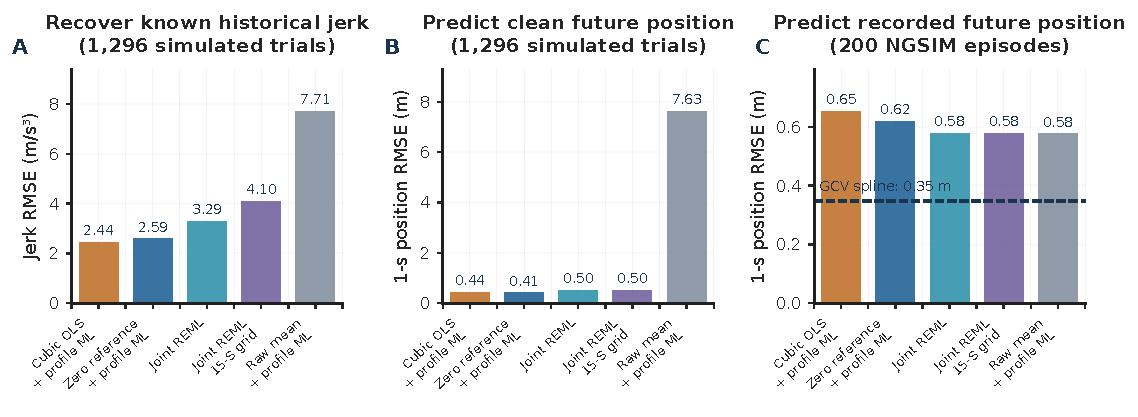
\includegraphics[width=\textwidth]{figures/exp006_reconstruction_forecasting.pdf}
\caption{Estimator choice depends on the
scientific outcome. (A) Known historical
discrete jerk RMSE on the archived
1,296-trajectory simulation.
(B) One-second forecast RMSE for
\emph{clean simulated future position}.
(C) One-second forecast RMSE for
\emph{recorded real NGSIM future position}
over 200 episodes, with GCV smoothing
spline reference marked. Panels are
different estimands with different
units and source populations;
they are not one pooled ranking.}
\label{fig:precision-endpoints}
\end{figure*}

The following simulation study asks
a separate question: does
the index $S$ measure a known
\emph{relative noise fraction}
when observation noise and genuine
jerk variability are manipulated
independently? This interpretation
cannot be assessed from forecast
RMSE or from visually smooth
jerk curves alone.
